\documentclass[15pt,a4paper]{report}
\usepackage[utf8]{vietnam}
\usepackage{amsmath}
\usepackage{amsfonts}
\usepackage{hyperref}
\usepackage{amsmath}
\usepackage{graphicx}
\usepackage{hyperref}
\usepackage{float} % Cần thiết cho tùy chọn [H]
\usepackage[utf8]{vietnam}
\usepackage{amsmath}
\usepackage{amsfonts}
\usepackage{amssymb}
\usepackage{graphicx}
\usepackage[left=1cm,right=1cm,top=1.5cm,bottom=1.5cm]{geometry}
\usepackage{blindtext}
\usepackage{titlesec}
\usepackage{graphicx}
\usepackage{multicol}
\usepackage{url}
\usepackage{matlab-prettifier}
\usepackage{caption}
\usepackage{arydshln}
\usepackage{mdframed}
\usepackage{amsthm}
\usepackage{listings}
\usepackage{xcolor}
\lstset{ 
	language=R,                % Ngôn ngữ
	basicstyle=\ttfamily\footnotesize, % Phông chữ
	%keywordstyle=\color{blue}, % Màu cho từ khóa
	commentstyle=\color{green!50!black}, % Màu cho chú thích
	stringstyle=\color{red},   % Màu cho chuỗi
	showstringspaces=false,    % Không hiển thị khoảng trắng trong chuỗi
	numbers=left,              % Hiển thị số dòng bên trái
	numberstyle=\tiny\color{gray}, % Phong chữ cho số dòng
	frame=single,              % Kẻ khung cho đoạn mã
	breaklines=true            % Tự động xuống dòng
}
\usepackage{graphicx}
\usepackage{pgfplots}
\fontsize{20pt}{15pt}
\usepgfplotslibrary{fillbetween}
\usetikzlibrary{patterns}


%%%%%%% code setup
\usepackage{listings}
\usepackage{caption}
\usepackage{xcolor}

% Không caption đánh số
\DeclareCaptionOption{lstlisting}{caption=false}{} 
\captionsetup[lstlisting]{labelformat=empty, position=bottom}

% (Tuỳ chọn) Màu nền nhẹ
\definecolor{mybg}{rgb}{0.94,0.94,0.94}

% Định nghĩa R
\lstdefinelanguage{R}{
	basicstyle=\ttfamily\small,
	keepspaces=true,
	showstringspaces=false,
	columns=fullflexible,
	upquote=true
}

% Định nghĩa Python
\lstdefinelanguage{Python}{
	basicstyle=\ttfamily\small,
	keepspaces=true,
	showstringspaces=false,
	columns=fullflexible,
	upquote=true
}

% Tắt hoàn toàn lề trái
\setlength{\parindent}{0pt}    % Không thụt lề đoạn văn
\setlength{\leftskip}{0pt}     % Không dịch trái toàn đoạn
\lstset{
	backgroundcolor=\color{mybg},
	breaklines=true,
	frame=none,
	numbers=none,
	xleftmargin=0pt,
	xrightmargin=0pt
}

%%%%%% end code setup

\begin{document}
\[
	\boxed{\huge \textbf{House Rent Analysis}}
\]
\section*{Data Preparation}
I have introduced the dataset \lstinline[language=R]|munichrent03| which is integrated in the R package \lstinline[language=R]|LinRegInteractive|, available at \href{https://github.com/taitran0102/rent-analysis/blob/main/README.md}{README.md} file. Therefore, I can simply load this dataset to begin the subsequent steps of the analysis.
\begin{lstlisting}[language=R]
library(LinRegInteractive)
data(munichrent03)
data <- munichrent03 
\end{lstlisting}
I began by examining the variable types to understand the structure of the dataset. 
\begin{lstlisting}[language=R]
> str(data)
'data.frame':	2053 obs. of  12 variables:
$ rent     : num  741 716 528 554 698 ...
$ rentsqm  : num  10.9 11.01 8.38 8.52 6.98 ...
$ area     : int  68 65 63 65 100 81 55 79 52 77 ...
$ rooms    : int  2 2 3 3 4 4 2 3 1 3 ...
$ yearc    : num  1918 1995 1918 1983 1995 ...
$ bathextra: Factor w/ 2 levels "no","yes": 1 1 1 2 2 1 2 1 1 1 ...
$ bathtile : Factor w/ 2 levels "yes","no": 1 1 1 1 1 1 1 1 1 1 ...
$ cheating : Factor w/ 2 levels "yes","no": 1 1 1 1 1 1 1 1 1 1 ...
$ district : Factor w/ 25 levels "All-Umenz","Alt-Le",..: 10 10 10 17 17 17 21 21 21 21 ...
$ location : Ord.factor w/ 3 levels "normal"<"good"<..: 2 2 2 1 2 1 1 1 1 1 ...
$ upkitchen: Factor w/ 2 levels "no","yes": 1 1 1 1 2 1 1 1 1 1 ...
$ wwater   : Factor w/ 2 levels "yes","no": 1 1 1 1 1 1 1 1 1 1 ...
> names(data)
'rent''rentsqm''area''rooms''yearc''bathextra''bathtile''cheating''district''location''upkitchen''wwater'
\end{lstlisting}
After that, I reviewed the distributions, value ranges, and identified any potential missing values.
\begin{lstlisting}[language=R]
> summary(data)
      rent            rentsqm            area           rooms      
Min.   :  77.31   Min.   : 1.470   Min.   : 17.0   Min.   :1.000  
1st Qu.: 389.95   1st Qu.: 6.800   1st Qu.: 53.0   1st Qu.:2.000  
Median : 534.30   Median : 8.470   Median : 67.0   Median :3.000  
Mean   : 570.09   Mean   : 8.394   Mean   : 69.6   Mean   :2.598  
3rd Qu.: 700.48   3rd Qu.:10.090   3rd Qu.: 83.0   3rd Qu.:3.000  
Max.   :1789.55   Max.   :20.090   Max.   :185.0   Max.   :6.000  

yearc      bathextra  bathtile   cheating        district      location   
Min.   :1918   no :1862   yes:1673   yes:1878   Neuh-Nymp: 177   normal:1205  
1st Qu.:1948   yes: 191   no : 380   no : 175   Lud-Isar : 161   good  : 803  
Median :1960                                    Au-Haid  : 139   top   :  45  
Mean   :1958                                    SchwWest : 137                
3rd Qu.:1973                                    Maxvor   : 132                
Max.   :2001                                    Laim     : 117                
(Other)  :1190                
upkitchen  wwater    
no :1903   yes:1981  
yes: 150   no :  72  

\end{lstlisting}
Note that the variables \lstinline[language=R]|rentsqm, rent| and \lstinline[language=R]|area| are related by the equation: \lstinline[language=R]|rent| = \lstinline[language=R]|rentsqm| $\times$ \lstinline[language=R]|area|. For example, at row 100, we have:

\begin{lstlisting}[language=R]
> round(data$rent[100]/data$area[100],2)  #compute rentsqm
11.3
> data$rentsqm[100]
11.3
\end{lstlisting}
Since \lstinline[language=R]|rentsqm| is a derived variable, I chose to exclude it and instead focus on total \lstinline[language=R]|rent|, which may better capture the underlying relationships with other features.
\begin{lstlisting}[language=R]
> data$rentsqm <- NULL
\end{lstlisting}
\section*{Exploratory Data Analysis}
Subsequently, I conducted an Exploratory Data Analysis (EDA) to gain initial insights into the dataset. A few key findings from this phase include:
\begin{itemize}
	\item The 7 districts with the largest number of houses
	\begin{lstlisting}[language=R]
Neuh-Nymp  Lud-Isar   Au-Haid  SchwWest    Maxvor      Laim   Ram-Per 
177        161        139       137        132         117       115 
	\end{lstlisting}
	\item The 7 districts with the highest number of houses where the location is classified as either “top” or “good”:
		\begin{lstlisting}[language=R]
Maxvor   Neuh-Nymp    Lud-Isar    SchwWest     Au-Haid Schwab-Frei    Trud-Rie 
118         116          97          96          81          50          37 
	\end{lstlisting}
	\item The proportion of houses equipped with each feature:
	\begin{lstlisting}[language=R]
    Feature Count Percent
1 bathextra   191     9.3
2  bathtile  1673    81.5
3  cheating  1878    91.5
4 upkitchen   150     7.3
5    wwater  1981    96.5
	\end{lstlisting}
	\item The distribution of the numerical variables in the dataset
	\begin{figure}[H]
		\centering 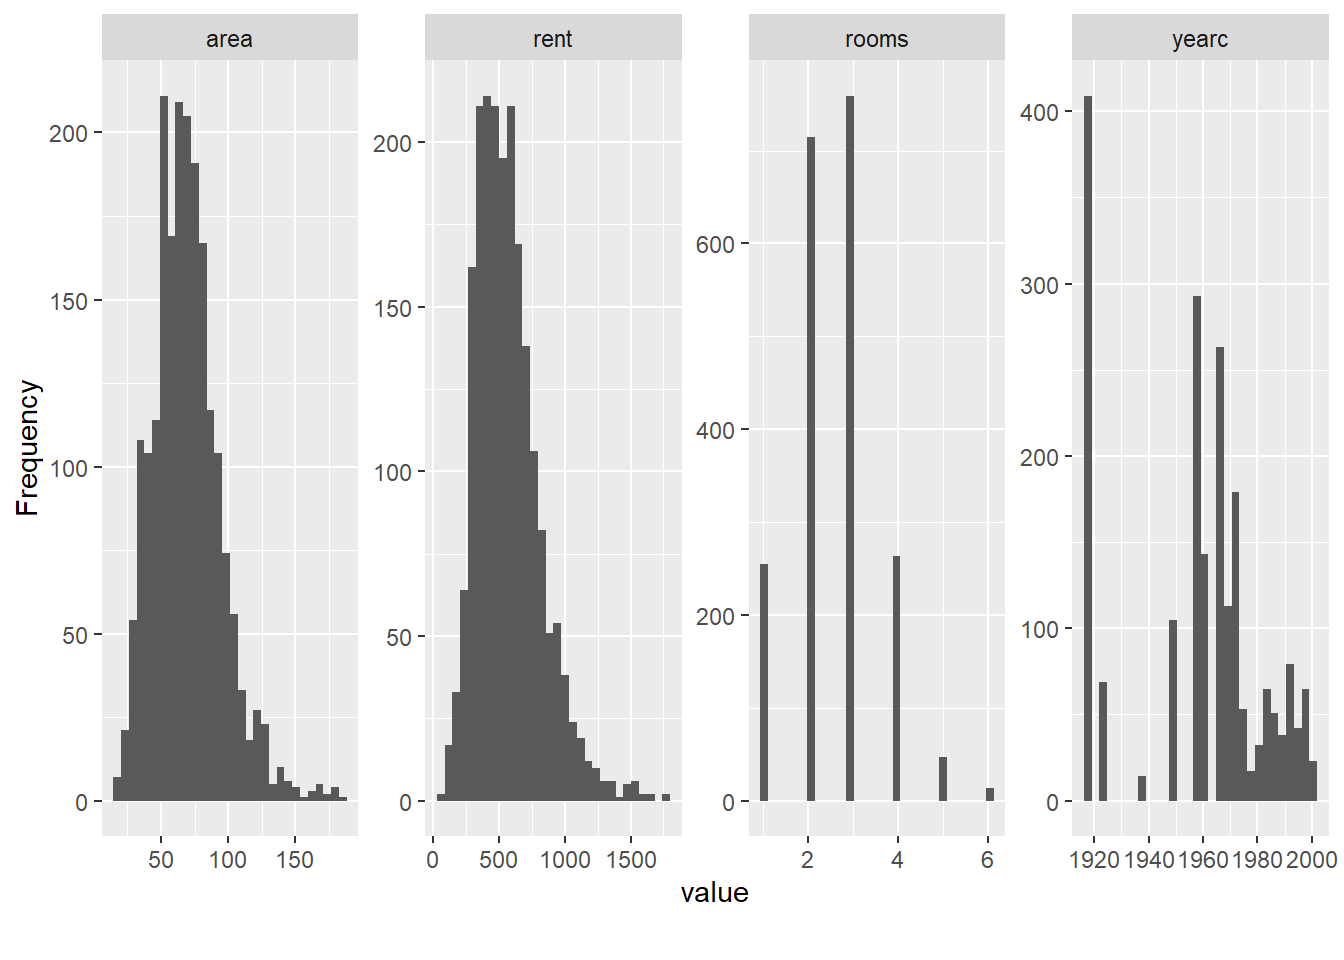
\includegraphics[width=\textwidth]{unnamed-chunk-10-1.png}
	\end{figure}
	\item The variable\lstinline[language=R]|yearc| represents discrete individual years, and the number of rooms(\lstinline[language=R]|room|)ranges only from 1 to 6.
		\begin{lstlisting}[language=R]
> table(data$room) #Count for each number of room

1   2   3   4   5   6 
255 715 759 263  47  14 
> table(data$yearc) #Count for each year

1918   1924   1939   1948   1957 1957.5   1960   1966   1967   1968 
409     69     14    105    225     68    143    228     35     23 
1969   1970   1971   1972   1973   1974   1975   1976   1977   1978 
44     46     35     89     55     30     16      7      6      5 
1979   1980   1981   1982   1983   1984   1985   1986   1987   1988 
6     17     15      8     40     17     20     11     20     13 
1989   1990   1991   1992   1993   1994   1995   1996   1997   1998 
15     10     14     24     41     13      9     20     12     14 
1998.5   1999   2000   2001 
32      7     18      5 
	\end{lstlisting}
\end{itemize}

\section*{Graphical Model Learning}
\section*{Inference and Querying}
\newpage

\[
\mathbb{P}(X<1,Y>1)=\int_{-\infty}^{1}\int_{1}^{+\infty}f(x,y) dx dy 
\]
\begin{figure}[H]
	\centering 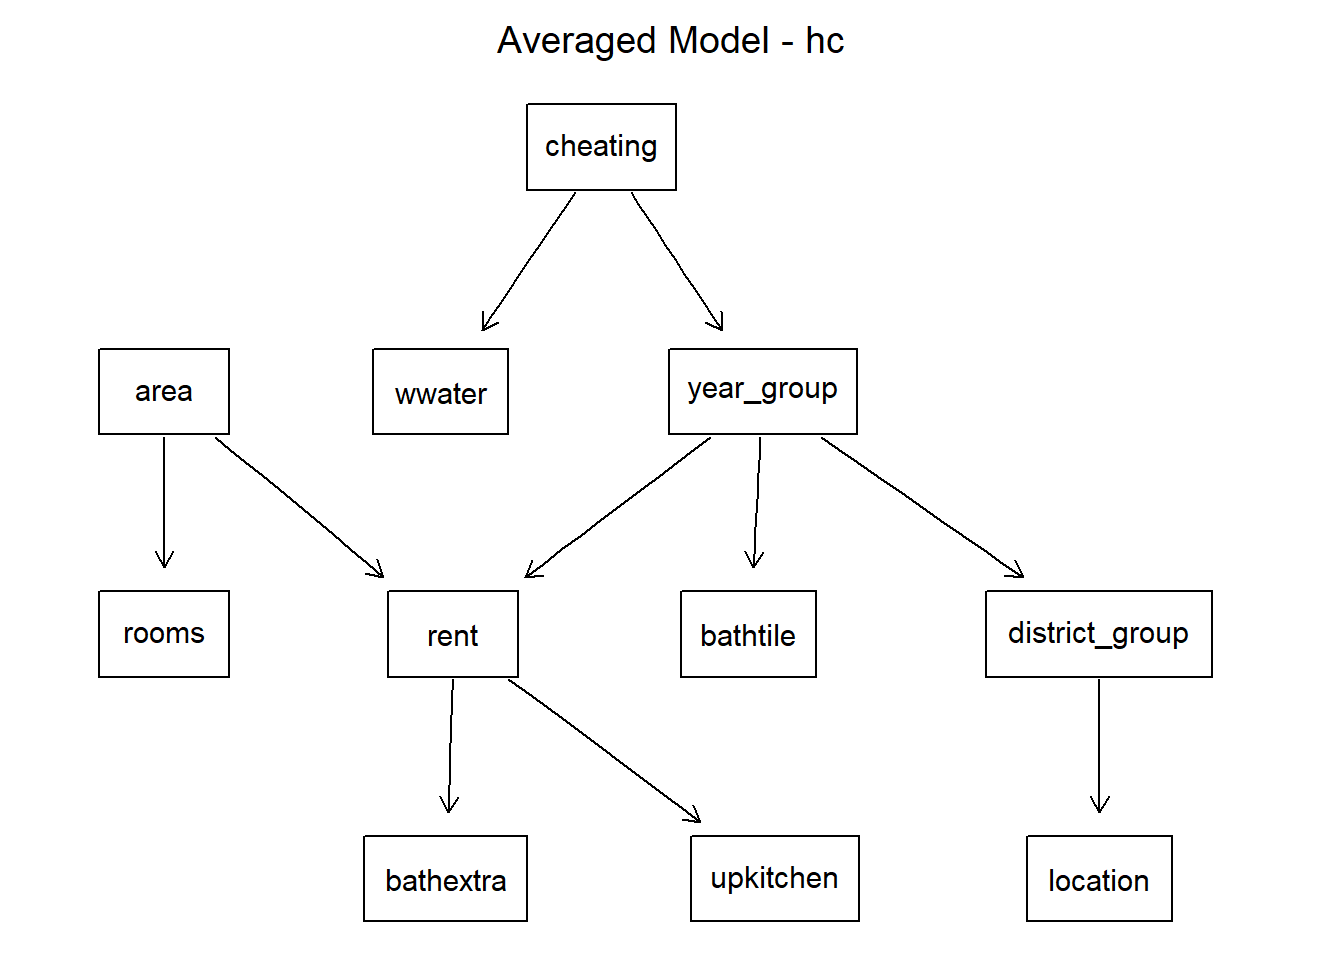
\includegraphics[width=0.6\textwidth]{unnamed-chunk-30-2.png}
\end{figure}
\end{document}